\documentclass[11pt,a4paper]{article}

\usepackage[utf8]{inputenc}
\usepackage[T1]{fontenc}
\usepackage{amsmath,amssymb,amsthm}
\usepackage{mathtools}
\usepackage{tikz}
\usetikzlibrary{trees,arrows.meta,positioning,decorations.pathmorphing,calc}
\usepackage{tikz-cd}
\usepackage{enumitem}
\usepackage{booktabs}
\usepackage{geometry}
\geometry{margin=2.5cm}
\usepackage{hyperref}
\hypersetup{colorlinks=true,linkcolor=blue!70!black,citecolor=green!50!black,urlcolor=blue!60!black}

% Theorem environments
\theoremstyle{plain}
\newtheorem{theorem}{Theorem}[section]
\newtheorem{proposition}[theorem]{Proposition}
\newtheorem{lemma}[theorem]{Lemma}
\newtheorem{corollary}[theorem]{Corollary}

\theoremstyle{definition}
\newtheorem{definition}[theorem]{Definition}
\newtheorem{example}[theorem]{Example}
\newtheorem{remark}[theorem]{Remark}

\theoremstyle{remark}
\newtheorem*{notation}{Notation}
\newtheorem*{caveat}{Caveat}
\newtheorem*{gap}{Honest Gap}

% Shortcuts
\newcommand{\HCK}{\mathcal{H}_{\mathrm{CK}}}
\newcommand{\GH}{G(\HCK)}
\renewcommand{\hbar}{\hslash}
\newcommand{\Lip}{\mathrm{Lip}}
\newcommand{\id}{\mathrm{id}}
\newcommand{\op}{\mathrm{op}}

% Tree drawing macros
\tikzset{
  treenode/.style = {circle, fill=black, inner sep=0pt, minimum size=5pt},
  treeedge/.style = {thick},
  subtraction/.style = {circle, draw=red, fill=red!20, inner sep=0pt, minimum size=7pt},
  counterterm/.style = {->, red!60!black, thick, decorate, decoration={snake, amplitude=1pt, segment length=4pt}},
}

\title{\textbf{The Cornerstone}:\\[6pt]
  Butcher Trees, Counterterm Subtraction,\\
  and the Forced Passage to Quantum Mechanics}

\author{Companion note to ``From Newton to the Path Integral''}

\date{February 2026}

\begin{document}
\maketitle

\begin{abstract}
We develop the identification that the rooted-tree algebra organising
Runge--Kutta order conditions is the \emph{same} algebra that organises
perturbative renormalisation, and that the passage from classical
mechanics to quantum mechanics is forced by requiring this
tree-organised counterterm subtraction to \emph{compose}.
Each edge of a Butcher tree encodes one derivative,
and each derivative is one counterterm subtraction.
The exact classical flow is the ``fully renormalised'' character of the
Connes--Kreimer Hopf algebra.
Quantisation extends the domain from one character to a weighted sum
over characters; the weight requires $\hbar > 0$ for the sum to
compose with an identity limit.
Renormalisation handles divergences in this sum using the same
coproduct that organised the original ODE order conditions.

We state this as a \emph{Cornerstone Proposition} (Proposition~\ref{prop:cornerstone}),
identify precisely what is a theorem and what remains conjectural,
and trace the three-level tree hierarchy
(Butcher $\to$ Frabetti $\to$ Hairer) that parallels the paper's
refinement chain (ODE $\to$ QM $\to$ QFT).
\end{abstract}

\tableofcontents

%% ===================================================================
\section{The derivative as a single counterterm subtraction}
\label{sec:derivative}
%% ===================================================================

\subsection{The regulated difference quotient}

Let $f:\mathbb{R}\to\mathbb{R}$ be continuous.
For a ``cutoff'' $\varepsilon > 0$, define the regulated quantities
\begin{equation}\label{eq:regulated}
  A_\varepsilon(x) := \frac{f(x+\varepsilon)}{\varepsilon},
  \qquad
  C_\varepsilon(x) := \frac{f(x)}{\varepsilon}.
\end{equation}
Both diverge as $\varepsilon\to 0$ whenever $f(x)\ne 0$.
The \textbf{renormalised} quantity is their difference:
\begin{equation}\label{eq:renormalized}
  R_\varepsilon(x)
  := A_\varepsilon(x) - C_\varepsilon(x)
  = \frac{f(x+\varepsilon) - f(x)}{\varepsilon}.
\end{equation}
If $f$ is differentiable at~$x$, the limit
$\lim_{\varepsilon\to 0} R_\varepsilon(x) = f'(x)$ exists and is finite:
the divergences cancel.

\begin{figure}[ht]
\centering
\begin{tikzpicture}[scale=1.2]
  % The divergent pieces
  \draw[->] (-0.5,0) -- (5,0) node[right] {$\varepsilon$};
  \draw[->] (0,-0.5) -- (0,4) node[above] {};

  % A_epsilon (diverges)
  \draw[blue, thick, domain=0.3:4.5, smooth, samples=50]
    plot (\x, {2/\x + 0.5}) node[right] {$A_\varepsilon = f(x{+}\varepsilon)/\varepsilon$};

  % C_epsilon (diverges)
  \draw[red, thick, domain=0.3:4.5, smooth, samples=50]
    plot (\x, {1.5/\x + 0.3}) node[right] {$C_\varepsilon = f(x)/\varepsilon$};

  % R_epsilon (converges)
  \draw[black!60!green, very thick, domain=0.3:4.5, smooth, samples=50]
    plot (\x, {0.5/\x + 0.2 + 0.8}) node[right] {$R_\varepsilon = f'(x) + O(\varepsilon)$};

  % The finite limit
  \draw[dashed, black!60!green] (0,1.0) -- (4.5,1.0);
  \node[left, black!60!green] at (0,1.0) {$f'(x)$};
\end{tikzpicture}
\caption{%
  Both $A_\varepsilon$ and $C_\varepsilon$ diverge as
  $\varepsilon\to 0$, but their difference $R_\varepsilon$
  converges to $f'(x)$.
  The ``counterterm'' $C_\varepsilon$ subtracts the local
  divergence, leaving a finite ``renormalised'' quantity.
}
\label{fig:divergence-cancellation}
\end{figure}

\subsection{The Lipschitz condition as uniform renormalisability}

\begin{proposition}\label{prop:lip-renorm}
  $f$ is Lipschitz with constant $L$ if and only if the renormalised
  quantity is uniformly bounded at all scales:
  \begin{equation}
    \sup_{x\in\mathbb{R},\;\varepsilon>0} |R_\varepsilon(x)| \le L.
  \end{equation}
\end{proposition}

This is the \textbf{zeroth-order RG condition}: the single-vertex
counterterm subtraction produces a bounded output at every scale
$\varepsilon > 0$.

\subsection{Graphical notation}

We represent this single counterterm subtraction as a vertex with
one incoming edge:

\begin{figure}[ht]
\centering
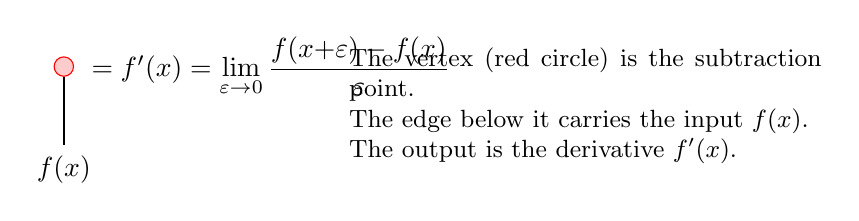
\begin{tikzpicture}
  % Single vertex
  \node[subtraction, label=right:{$\;= f'(x) = \displaystyle\lim_{\varepsilon\to 0}
    \frac{f(x{+}\varepsilon)-f(x)}{\varepsilon}$}] (v) at (0,0) {};
  \draw[treeedge] (v) -- ++(0,-1) node[below] {$f(x)$};

  \node[anchor=west] at (3.5,-0.5) {%
    \begin{minipage}{6cm}
    \small
    The vertex (red circle) is the subtraction point.\\
    The edge below it carries the input $f(x)$.\\
    The output is the derivative $f'(x)$.
    \end{minipage}
  };
\end{tikzpicture}
\caption{A single counterterm subtraction = one derivative.}
\label{fig:single-vertex}
\end{figure}


%% ===================================================================
\section{Trees as iterated counterterm subtractions}
\label{sec:trees}
%% ===================================================================

\subsection{The first Butcher trees}

For the ODE $\dot{y} = f(y)$, the Taylor expansion of the exact flow
$\Phi_h(y)$ is indexed by rooted trees.
Each tree prescribes a pattern of nested derivatives of $f$.
Since each derivative is a counterterm subtraction (Section~\ref{sec:derivative}),
\textbf{each tree is a pattern of nested counterterm subtractions}.

\begin{figure}[ht]
\centering
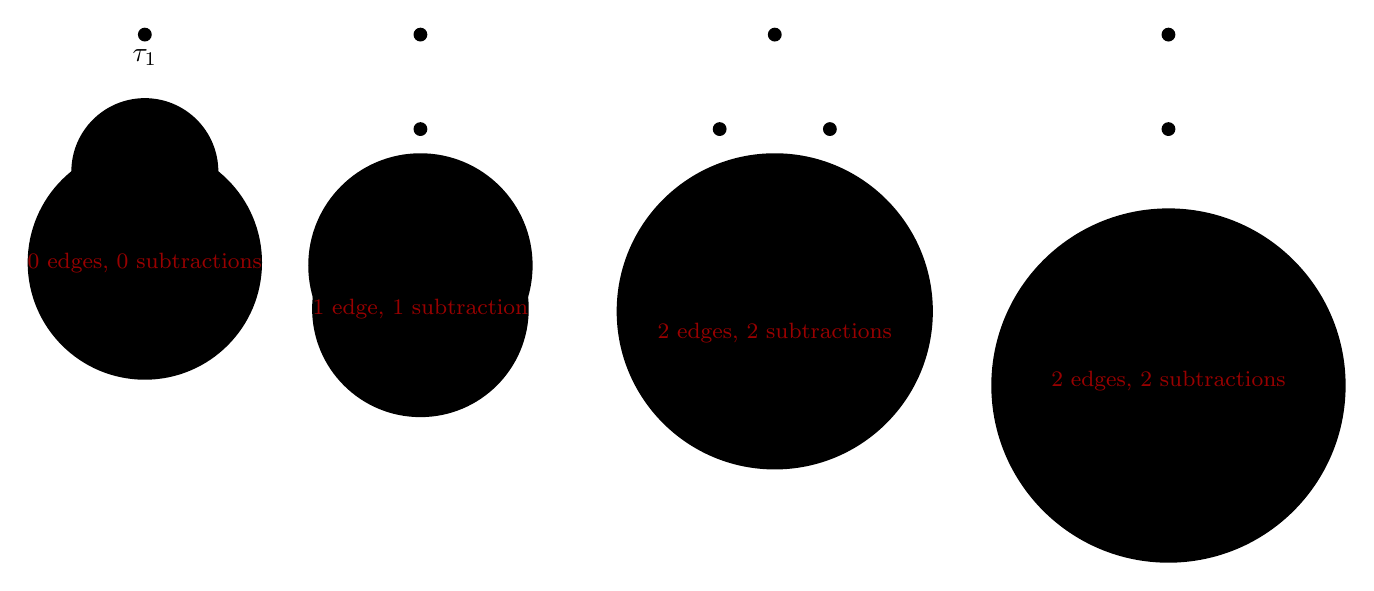
\begin{tikzpicture}[
  level distance=12mm,
  sibling distance=14mm,
  every node/.style={treenode},
  edge from parent/.style={treeedge}
]

% tau_1: single vertex
\begin{scope}[xshift=0cm]
  \node[treenode, label=below:{$\tau_1$}] (t1) {};
  \node[anchor=north, font=\small] at (0,-0.8) {$F(\tau_1) = f(y)$};
  \node[anchor=north, font=\footnotesize, text=red!60!black] at (0,-1.4) {0 edges, 0 subtractions};
\end{scope}

% tau_2: chain of 2
\begin{scope}[xshift=3.5cm]
  \node[treenode, label=left:{}] (a) {}
    child { node[treenode] {} };
  \node[anchor=north, font=\small] at (0,-1.5) {$F(\tau_2) = f'(y)\bigl[f(y)\bigr]$};
  \node[anchor=north, font=\footnotesize, text=red!60!black] at (0,-2.1) {1 edge, 1 subtraction};
  \node[below=0.3cm, font=\small] at (0,-2.5) {$\tau_2$};
\end{scope}

% tau_3a: branch
\begin{scope}[xshift=8cm]
  \node[treenode] (b) {}
    child { node[treenode] {} }
    child { node[treenode] {} };
  \node[anchor=north, font=\small, text width=4cm, align=center] at (0,-1.5)
    {$F(\tau_{3a}) = f''(y)\bigl[f(y),f(y)\bigr]$};
  \node[anchor=north, font=\footnotesize, text=red!60!black] at (0,-2.3) {2 edges, 2 subtractions};
  \node[below=0.3cm, font=\small] at (0,-2.7) {$\tau_{3a}$};
\end{scope}

% tau_3b: chain of 3
\begin{scope}[xshift=13cm]
  \node[treenode] (c) {}
    child { node[treenode] {}
      child { node[treenode] {} }
    };
  \node[anchor=north, font=\small, text width=4.5cm, align=center] at (0,-2.2)
    {$F(\tau_{3b}) = f'(y)\bigl[f'(y)[f(y)]\bigr]$};
  \node[anchor=north, font=\footnotesize, text=red!60!black] at (0,-2.9) {2 edges, 2 subtractions};
  \node[below=0.3cm, font=\small] at (0,-3.3) {$\tau_{3b}$};
\end{scope}

\end{tikzpicture}
\caption{%
  The first four Butcher trees (orders 1--3) with their elementary
  differentials.
  Each \textbf{edge} represents one application of a derivative of $f$,
  which is one counterterm subtraction.
  The number of edges equals the number of subtractions: $|\tau|-1$.
}
\label{fig:first-trees}
\end{figure}


\subsection{The order-4 trees}

At order 4 there are four distinct (unordered) rooted trees.
They exhaust the ways to nest three counterterm subtractions:

\begin{figure}[ht]
\centering
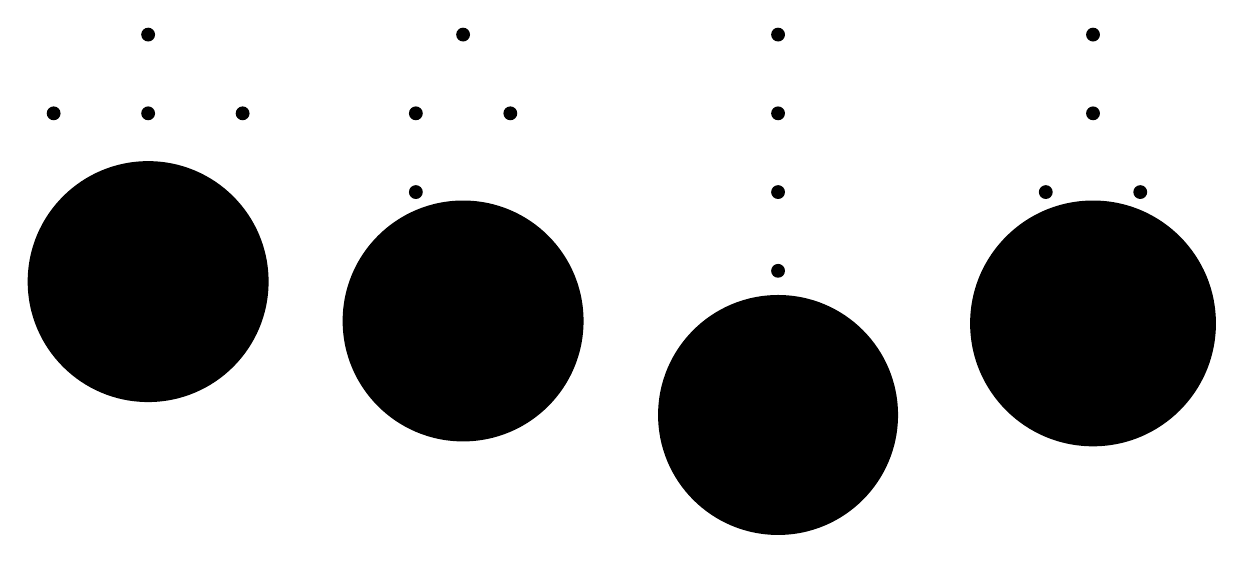
\begin{tikzpicture}[
  level distance=10mm,
  sibling distance=12mm,
  every node/.style={treenode},
  edge from parent/.style={treeedge}
]

% tau_4a: star (root with 3 children)
\begin{scope}[xshift=0cm]
  \node[treenode] {}
    child { node[treenode] {} }
    child { node[treenode] {} }
    child { node[treenode] {} };
  \node[font=\footnotesize, anchor=north, text width=3cm, align=center] at (0,-1.6)
    {$f'''[f,f,f]$\\3 parallel subtractions};
  \node[font=\small] at (0,-2.6) {$\tau_{4a}$};
\end{scope}

% tau_4b: root->branch
\begin{scope}[xshift=4cm]
  \node[treenode] {}
    child { node[treenode] {}
      child { node[treenode] {} }
    }
    child { node[treenode] {} };
  \node[font=\footnotesize, anchor=north, text width=3cm, align=center] at (0,-2.1)
    {$f''[f'[f],f]$\\serial + parallel};
  \node[font=\small] at (0,-3.1) {$\tau_{4b}$};
\end{scope}

% tau_4c: root->chain->leaf + leaf (this is same as 4b up to tree iso for unordered)
% Actually for unordered trees tau_4b already covers this. Let me do the chain of 4.

% tau_4c: chain of 4
\begin{scope}[xshift=8cm]
  \node[treenode] {}
    child { node[treenode] {}
      child { node[treenode] {}
        child { node[treenode] {} }
      }
    };
  \node[font=\footnotesize, anchor=north, text width=3cm, align=center] at (0,-3.3)
    {$f'[f'[f'[f]]]$\\3 serial subtractions};
  \node[font=\small] at (0,-4.3) {$\tau_{4c}$};
\end{scope}

% tau_4d: root -> (vertex with 2 children)
\begin{scope}[xshift=12cm]
  \node[treenode] {}
    child { node[treenode] {}
      child { node[treenode] {} }
      child { node[treenode] {} }
    };
  \node[font=\footnotesize, anchor=north, text width=3cm, align=center] at (0,-2.1)
    {$f'[f''[f,f]]$\\inner parallel,\\outer serial};
  \node[font=\small] at (0,-3.3) {$\tau_{4d}$};
\end{scope}

\end{tikzpicture}
\caption{%
  The four order-4 Butcher trees.
  Each has 3 edges = 3 counterterm subtractions.
  The topology determines \emph{how} the subtractions are composed:
  all-parallel ($\tau_{4a}$),
  mixed ($\tau_{4b}$, $\tau_{4d}$),
  or all-serial ($\tau_{4c}$).
}
\label{fig:order4-trees}
\end{figure}

\subsection{The general count}

\begin{proposition}\label{prop:edge-count}
  For a rooted tree $\tau$ with $|\tau|$ vertices:
  \begin{enumerate}[label=(\roman*)]
    \item The number of edges is $|\tau|-1$.
    \item Each edge encodes one application of a derivative of $f$,
      which is one counterterm subtraction.
    \item The total ``subtraction depth'' of the tree is
      $\sum_{v\in\tau} k_v = |\tau|-1$,
      where $k_v$ is the number of children of vertex $v$.
  \end{enumerate}
\end{proposition}

\begin{proof}
  Every tree on $n$ vertices has exactly $n-1$ edges.
  Each edge connects a child to its parent; the parent vertex
  applies $f^{(k_v)}[\cdot,\ldots,\cdot]$ where $k_v$ is its
  number of children.
  Since $f^{(k)}$ involves $k$ limiting subtractions
  (each partial derivative is a limit of a difference quotient),
  the total is $\sum_v k_v = |\tau|-1$.
\end{proof}


%% ===================================================================
\section{The exact flow as the fully renormalised character}
\label{sec:exact-flow}
%% ===================================================================

\subsection{The Butcher B-series}

The Taylor expansion of the exact flow $\Phi_h(y)$ of $\dot{y}=f(y)$
is the \textbf{B-series}:
\begin{equation}\label{eq:bseries}
  \Phi_h(y) = y + \sum_{\tau\in\mathcal{T}}
  \frac{h^{|\tau|}}{\sigma(\tau)}\,F(\tau)(y),
\end{equation}
where $\mathcal{T}$ is the set of rooted trees,
$|\tau|$ is the order (number of vertices),
$\sigma(\tau)$ is a symmetry factor
($\sigma(\tau_1)=1$, $\sigma(\tau_2)=2$, $\sigma(\tau_{3a})=3$,
$\sigma(\tau_{3b})=6$, \ldots),
and $F(\tau)$ is the elementary differential (Figures~\ref{fig:first-trees}--\ref{fig:order4-trees}).

\subsection{Characters of the Hopf algebra}

The Connes--Kreimer Hopf algebra $\HCK$ is the commutative polynomial
algebra generated by rooted trees, with coproduct $\Delta$ defined
by admissible cuts (Section~\ref{sec:coproduct}).

\begin{definition}
  A \textbf{character} of $\HCK$ is an algebra homomorphism
  $\phi:\HCK\to\mathbb{R}$.
  It assigns a coefficient $\phi(\tau)\in\mathbb{R}$ to each tree.
  The set of all characters forms a group $\GH$ under the
  convolution product $\star$ (the \textbf{Butcher group}).
\end{definition}

\begin{definition}
  The \textbf{exact-flow character} is
  $\phi_{\mathrm{exact}}(\tau) := 1/\sigma(\tau)$.
\end{definition}

\begin{theorem}[Butcher 1972]
  \label{thm:butcher-order}
  A Runge--Kutta method with Butcher tableau $(A,b,c)$ defines
  a character $\phi_{\mathrm{RK}}$ via
  $\phi_{\mathrm{RK}}(\tau) = \Phi_\tau(A,b,c)$
  (a polynomial in the tableau entries).
  The method has order $p$ if and only if
  \begin{equation}
    \phi_{\mathrm{RK}}(\tau) = \phi_{\mathrm{exact}}(\tau)
    \quad\text{for all } |\tau| \le p.
  \end{equation}
\end{theorem}

\begin{remark}[The exact flow is ``fully renormalised'']
  The exact-flow character $\phi_{\mathrm{exact}}$ is the unique element
  of $\GH$ that gets \emph{every} counterterm subtraction right at
  \emph{every} order.
  A numerical method of order $p$ gets them right up to order $p$;
  the discrepancy $\delta_\tau := \phi_{\mathrm{RK}}(\tau) - 1/\sigma(\tau)$
  at order $p+1$ is the \textbf{counterterm} needed to correct the method.
\end{remark}

\subsection{The control map as a counterterm}

The main paper's Derivation D6.2a defines the step-halving comparison:
compose two half-steps $\Phi_{h/2}\circ\Phi_{h/2}$ and compare with
$\Phi_h$.
In the family $\Phi_h^{(a)}(y) = y + hf(y) + ah^2 f'(y)[f(y)] + O(h^3)$,
this gives
\begin{equation}
  \Phi_{h/2}^{(a)}\circ\Phi_{h/2}^{(a)}
  = \Phi_h^{(\tau_2(a))} + O(h^3),
  \qquad
  \tau_2(a) = \frac{a}{2} + \frac{1}{4}.
\end{equation}

\begin{figure}[ht]
\centering
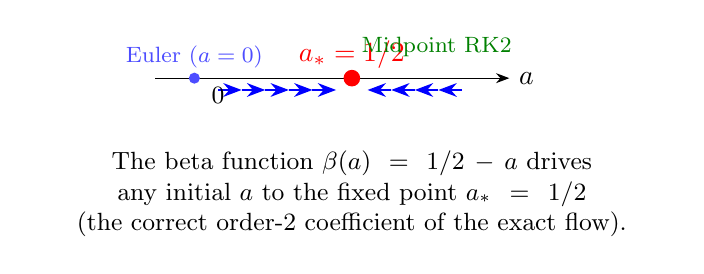
\begin{tikzpicture}[>=Stealth]
  % The a-axis
  \draw[->] (-0.5,0) -- (4,0) node[right] {$a$};

  % Fixed point
  \fill[red] (2,0) circle (3pt) node[above] {$a_* = 1/2$};

  % Flow arrows
  \foreach \x in {0.3, 0.6, 0.9, 1.2, 1.5} {
    \draw[->, thick, blue] (\x, -0.15) -- (\x+0.3, -0.15);
  }
  \foreach \x in {2.5, 2.8, 3.1, 3.4} {
    \draw[->, thick, blue] (\x, -0.15) -- (\x-0.3, -0.15);
  }

  % Labels
  \node[below, font=\small] at (0.3,0) {$0$};
  \node[below, font=\small] at (3.5,0) {};
  \node[below=0.5cm, font=\small, text width=8cm, align=center] at (2,-0.3)
    {The beta function $\beta(a) = 1/2 - a$ drives\\
     any initial $a$ to the fixed point $a_* = 1/2$\\
     (the correct order-2 coefficient of the exact flow).};

  % Explicit Euler
  \fill[blue!70] (0,0) circle (2pt) node[above, font=\footnotesize] {Euler ($a=0$)};

  % Midpoint
  \fill[green!50!black] (2,0) circle (0pt);
  \node[above right, font=\footnotesize, green!50!black] at (2,0.15) {Midpoint RK2};
\end{tikzpicture}
\caption{%
  The control map $\tau_2(a) = a/2 + 1/4$ on the parameter space
  of order-2 coefficients.
  This is the counterterm for the single tree $\tau_2 = $~(chain of 2).
  The fixed point $a_* = 1/2$ is the exact-flow value.
  Repeated halving drives any initial method toward the exact flow.
}
\label{fig:control-map}
\end{figure}

In the Hopf-algebraic language: $\tau_2(a)$ is the $|\tau|=2$
component of the Butcher group product
$\phi_{h/2}\star\phi_{h/2}$ projected onto the one-parameter
family.
The full tree-level comparison would give a control map
$\tau_b^{(\tau)}$ for \emph{each} tree $\tau$, with the
semigroup property
$\tau_b^{(\tau)}\circ\tau_c^{(\tau)} = \tau_{bc}^{(\tau)}$
inherited from the group law of $\GH$.


%% ===================================================================
\section{The coproduct: same structure for ODEs and QFT}
\label{sec:coproduct}
%% ===================================================================

\subsection{Admissible cuts}

The coproduct $\Delta:\HCK\to\HCK\otimes\HCK$ is defined by
\textbf{admissible cuts}: remove a subset of edges from the tree
such that at most one edge on each root-to-leaf path is cut.
The pieces below the cuts form the ``pruned part'' $P^c(\tau)$
(a forest of subtrees), and the piece containing the root is
the ``trunk'' $R^c(\tau)$.

\begin{equation}\label{eq:coproduct}
  \Delta(\tau) = \tau\otimes\mathbf{1}
  + \mathbf{1}\otimes\tau
  + \sum_{\text{admissible cuts } c} P^c(\tau)\otimes R^c(\tau).
\end{equation}

\subsection{Worked example: $\Delta(\tau_2)$}

\begin{figure}[ht]
\centering
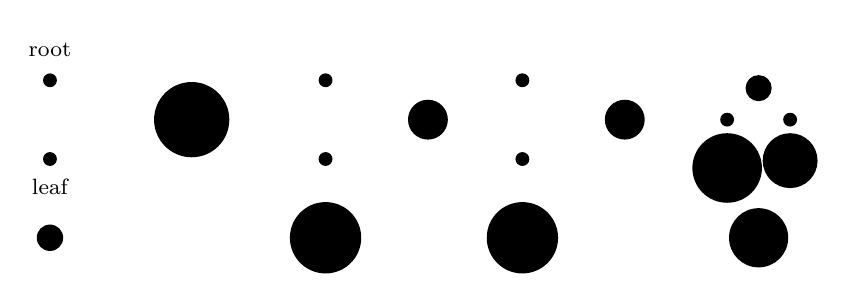
\begin{tikzpicture}[
  level distance=10mm,
  every node/.style={treenode},
  edge from parent/.style={treeedge}
]

% Original tree
\begin{scope}[xshift=0cm]
  \node[treenode, label=above:{\footnotesize root}] (a) {}
    child { node[treenode, label=below:{\footnotesize leaf}] {} };
  \node[font=\small] at (0,-2) {$\tau_2$};
\end{scope}

\node[font=\Large] at (1.8,-0.5) {$\xmapsto{\;\Delta\;}$};

% Term 1: tau_2 x 1
\begin{scope}[xshift=3.5cm]
  \node[treenode] {}
    child { node[treenode] {} };
  \node[font=\small] at (0,-2) {$\tau_2\otimes\mathbf{1}$};
\end{scope}

\node[font=\Large] at (4.8,-0.5) {$+$};

% Term 2: 1 x tau_2
\begin{scope}[xshift=6cm]
  \node[treenode] {}
    child { node[treenode] {} };
  \node[font=\small] at (0,-2) {$\mathbf{1}\otimes\tau_2$};
\end{scope}

\node[font=\Large] at (7.3,-0.5) {$+$};

% Term 3: bullet x bullet (the one admissible cut)
\begin{scope}[xshift=9cm]
  \node[treenode] (p) at (-0.4, -0.5) {};
  \node[font=\scriptsize, below=2pt of p] {pruned};
  \node[font=\small] at (0,-0.1) {$\otimes$};
  \node[treenode] (t) at (0.4, -0.5) {};
  \node[font=\scriptsize, below=2pt of t] {trunk};
  \node[font=\small] at (0,-2) {$\bullet\otimes\bullet$};
\end{scope}

\end{tikzpicture}
\caption{%
  The coproduct of the chain tree $\tau_2$.
  There is one non-trivial admissible cut (cutting the single edge),
  which separates the leaf (pruned: $\bullet = f$) from the
  root (trunk: $\bullet = f'[\cdot]$ waiting for input).
}
\label{fig:coproduct-tau2}
\end{figure}

\subsection{Worked example: $\Delta(\tau_{3b})$}

The chain of three has two edges and hence more admissible cuts:

\begin{figure}[ht]
\centering
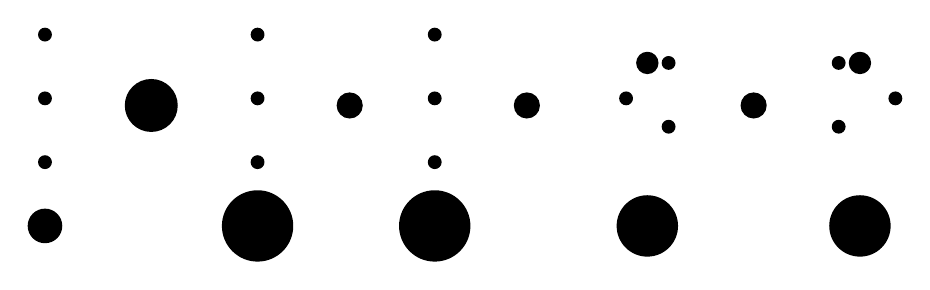
\begin{tikzpicture}[
  level distance=9mm,
  every node/.style={treenode},
  edge from parent/.style={treeedge},
  scale=0.9
]

% Original
\begin{scope}[xshift=0cm]
  \node[treenode] {} child { node[treenode] {} child { node[treenode] {} } };
  \node[font=\small] at (0,-2.7) {$\tau_{3b}$};
\end{scope}

\node[font=\small] at (1.5,-1) {$\xmapsto{\;\Delta\;}$};

% tau_{3b} x 1
\begin{scope}[xshift=3cm]
  \node[treenode] {} child { node[treenode] {} child { node[treenode] {} } };
  \node[font=\scriptsize] at (0,-2.7) {$\tau_{3b}\otimes\mathbf{1}$};
\end{scope}

\node[font=\small] at (4.3,-1) {$+$};

% 1 x tau_{3b}
\begin{scope}[xshift=5.5cm]
  \node[treenode] {} child { node[treenode] {} child { node[treenode] {} } };
  \node[font=\scriptsize] at (0,-2.7) {$\mathbf{1}\otimes\tau_{3b}$};
\end{scope}

\node[font=\small] at (6.8,-1) {$+$};

% Cut bottom edge: bullet x tau_2
\begin{scope}[xshift=8.5cm]
  \node[treenode] at (-0.3,-0.9) {};
  \node[font=\scriptsize] at (0,-0.4) {$\otimes$};
  \node[treenode] (r1) at (0.3,-0.4) {}
    child { node[treenode] {} };
  \node[font=\scriptsize] at (0,-2.7) {$\bullet\otimes\tau_2$};
\end{scope}

\node[font=\small] at (10,-1) {$+$};

% Cut top edge: tau_2 x bullet
\begin{scope}[xshift=11.5cm]
  \node[treenode] (l1) at (-0.3,-0.4) {}
    child { node[treenode] {} };
  \node[font=\scriptsize] at (0,-0.4) {$\otimes$};
  \node[treenode] at (0.5,-0.9) {};
  \node[font=\scriptsize] at (0,-2.7) {$\tau_2\otimes\bullet$};
\end{scope}

\end{tikzpicture}
\caption{%
  The coproduct of the chain $\tau_{3b}$.
  Two admissible cuts yield $\bullet\otimes\tau_2$ (cut bottom edge)
  and $\tau_2\otimes\bullet$ (cut top edge).
  Cutting both edges simultaneously is \emph{not} admissible
  (it would cut two edges on the same root-to-leaf path).
}
\label{fig:coproduct-tau3b}
\end{figure}


\subsection{The dual interpretation}

\begin{center}
\renewcommand{\arraystretch}{1.4}
\begin{tabular}{p{5.5cm}p{5.5cm}}
\toprule
\textbf{ODE / Runge--Kutta} & \textbf{QFT / Renormalisation} \\
\midrule
Admissible cut separates a
sub-pattern of derivatives
& Admissible cut separates a
divergent subdiagram \\
Pruned part = inner composition step
& Pruned part = subdivergence \\
Trunk = outer composition step
& Trunk = reduced diagram \\
$(\phi\star\psi)(\tau) = \sum \phi(P^c)\psi(R^c)$:
compose two flows
& Same formula: compose renormalisation maps \\
Order conditions:
$\phi_{\mathrm{RK}}(\tau)=1/\sigma(\tau)$
& Renormalisation conditions:
$\phi_+(\tau) = $ finite part \\
\bottomrule
\end{tabular}
\end{center}

This is the content of Brouder's theorem (1999):
the Butcher group and the Connes--Kreimer renormalisation group
are the \textbf{same group} $\GH$.


%% ===================================================================
\section{From one character to all: why $\hbar$ enters}
\label{sec:quantization}
%% ===================================================================

\subsection{The classical situation}

Classically, the flow $\Phi_t$ is deterministic.
Given $y_0$, there is one trajectory $y(t) = \Phi_t(y_0)$.
The B-series \eqref{eq:bseries} computes this single trajectory.
All trees contribute, but to a \textbf{single} character $\phi_{\mathrm{exact}}$.

\subsection{The compositional question}

Now ask: can the flow be represented as a smooth \textbf{transition kernel}
$K(x,y;t)$ satisfying
\begin{equation}\label{eq:composition}
  K(x,y;\,t_1{+}t_2) = \int K(x,z;\,t_1)\,K(z,y;\,t_2)\,dz
\end{equation}
with the identity limit $K(x,y;t)\to\delta(x{-}y)$ as $t\to 0^+$?

The classical answer $K_{\mathrm{cl}}(x,y;t) = \delta(y-\Phi_t(x))$
satisfies \eqref{eq:composition} but is not smooth.

\subsection{The smooth obstruction (P4.2)}

If we require $K$ to be a smooth function (not a distribution), then
the main paper's Proposition P4.2 shows:

\begin{enumerate}[label=(\alph*)]
  \item Composition closure on smooth kernels forces the normalisation
    $K \propto t^{-d/2}$.
  \item The identity limit forces an exponential weight
    $K \propto \exp\bigl(-Q(x,y)/(\kappa t)\bigr)$
    with $[\kappa] = [\text{action}]$.
  \item Setting $\kappa\to 0$ concentrates $K$ on $\delta(y-\Phi_t(x))$,
    but the identity limit is lost for $t > 0$
    (the flow $\Phi_t$ is not the identity for $t>0$).
  \item Therefore $\kappa = \hbar > 0$ is forced.
\end{enumerate}

\begin{figure}[ht]
\centering
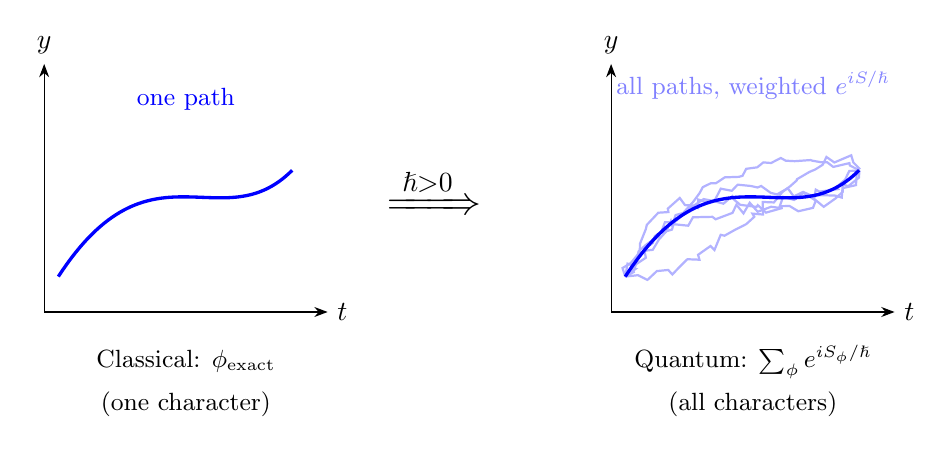
\begin{tikzpicture}[>=Stealth, scale=0.9]
  % Classical: one path
  \begin{scope}[xshift=0cm]
    \draw[->] (0,0) -- (0,3.5) node[above] {$y$};
    \draw[->] (0,0) -- (4,0) node[right] {$t$};
    \draw[very thick, blue] (0.2,0.5) .. controls (1.5,2.5) and (2.5,1.0) .. (3.5,2.0);
    \node[font=\small, blue] at (2,3) {one path};
    \node[font=\small] at (2,-0.7) {Classical: $\phi_{\mathrm{exact}}$};
    \node[font=\small] at (2,-1.3) {(one character)};
  \end{scope}

  % Arrow
  \node[font=\Large] at (5.5,1.5) {$\xRightarrow{\;\hbar > 0\;}$};

  % Quantum: sum over paths
  \begin{scope}[xshift=8cm]
    \draw[->] (0,0) -- (0,3.5) node[above] {$y$};
    \draw[->] (0,0) -- (4,0) node[right] {$t$};

    % Multiple wiggly paths
    \draw[blue!30, thick, decorate, decoration={random steps, segment length=3pt, amplitude=2pt}]
      (0.2,0.5) .. controls (1,2.8) and (2.5,0.5) .. (3.5,2.0);
    \draw[blue!30, thick, decorate, decoration={random steps, segment length=3pt, amplitude=2pt}]
      (0.2,0.5) .. controls (0.8,1.5) and (2,2.5) .. (3.5,2.0);
    \draw[blue!30, thick, decorate, decoration={random steps, segment length=3pt, amplitude=2pt}]
      (0.2,0.5) .. controls (1.5,0.3) and (3,2.8) .. (3.5,2.0);
    \draw[blue!30, thick, decorate, decoration={random steps, segment length=3pt, amplitude=2pt}]
      (0.2,0.5) .. controls (1,1.8) and (2.5,1.2) .. (3.5,2.0);
    \draw[blue!30, thick, decorate, decoration={random steps, segment length=3pt, amplitude=2pt}]
      (0.2,0.5) .. controls (2,3.0) and (3,0.8) .. (3.5,2.0);

    % The classical path (dominant)
    \draw[very thick, blue] (0.2,0.5) .. controls (1.5,2.5) and (2.5,1.0) .. (3.5,2.0);

    \node[font=\small, blue!50] at (2,3.2) {all paths, weighted $e^{iS/\hbar}$};
    \node[font=\small] at (2,-0.7) {Quantum: $\sum_\phi e^{iS_\phi/\hbar}$};
    \node[font=\small] at (2,-1.3) {(all characters)};
  \end{scope}
\end{tikzpicture}
\caption{%
  Classical mechanics uses one character (the extremal path).
  Quantum mechanics sums over all characters, weighted by $e^{iS/\hbar}$.
  The classical limit $\hbar\to 0$ projects back to the dominant
  (stationary-phase) character.
  Composition \eqref{eq:composition} forces $\hbar > 0$.
}
\label{fig:classical-vs-quantum}
\end{figure}

\subsection{The tree-level reading}

In the perturbative expansion, the quantum propagator decomposes as
\begin{equation}
  K(x,y;t) \sim K_0(x,y;t)\,\biggl(
    1 + \sum_{n=1}^\infty \hbar^n \sum_{|\tau|=n+1}
    c_\tau\,F(\tau)(x,y)
  \biggr),
\end{equation}
where $K_0$ is the free (Gaussian) kernel and the $c_\tau$ are
combinatorial coefficients.
The trees that appear are the \emph{same} Butcher trees,
but now they index the perturbative corrections to the propagator
rather than the Taylor corrections to the ODE flow.

\begin{center}
\renewcommand{\arraystretch}{1.4}
\begin{tabular}{lll}
\toprule
& \textbf{Classical (ODE)} & \textbf{Quantum (path integral)} \\
\midrule
Character & one: $\phi_{\mathrm{exact}}$ & all: $\sum_\phi e^{iS_\phi/\hbar}$ \\
Expansion parameter & $h$ (step size) & $\hbar$ (action scale) \\
Trees index & Taylor corrections & perturbative corrections \\
$\hbar\to 0$ limit & --- & stationary phase $\to\phi_{\mathrm{exact}}$ \\
Lipschitz condition & $\|f'\|\le L_0$ (well-posedness) & $V\in\mathcal{K}_d$ (Kato class) \\
\bottomrule
\end{tabular}
\end{center}


%% ===================================================================
\section{The Cornerstone Proposition}
\label{sec:cornerstone}
%% ===================================================================

\begin{proposition}[Cornerstone]
\label{prop:cornerstone}
Let $\HCK$ be the Connes--Kreimer Hopf algebra of rooted trees
and $\GH$ its group of characters (the Butcher group).

\begin{enumerate}[label=\textbf{(\roman*)}]
  \item \textbf{Trees = organised subtractions.}
    The exact flow $\Phi_t$ of $\dot{y}=f(y)$ defines a character
    $\phi_{\mathrm{exact}}\in\GH$ via $\phi_{\mathrm{exact}}(\tau)=1/\sigma(\tau)$.
    Each edge of $\tau$ encodes one derivative of $f$,
    which is one counterterm subtraction (D6.3).
    A Runge--Kutta method of order $p$ is a character $\phi_{\mathrm{RK}}$
    agreeing with $\phi_{\mathrm{exact}}$ on $|\tau|\le p$;
    the discrepancy $\delta_\tau$ at order $p+1$ is a counterterm.

  \item \textbf{Composition = Hopf product.}
    The composition $\Phi_s\circ\Phi_t$ corresponds to the convolution
    product $\phi_s\star\phi_t$ in $\GH$,
    defined via the coproduct $\Delta$.
    The control map $\tau_b$ of D6.2a is the $|\tau|=2$ truncation.
    The semigroup $\tau_b\circ\tau_c = \tau_{bc}$ is a shadow of the
    group law of $\GH$.

  \item \textbf{Composition forces $\hbar$.}
    When the transition kernel $K(x,y;t)$ is required to be smooth,
    compose via~\eqref{eq:composition}, and satisfy $K\to\delta$ as
    $t\to 0^+$, then $K$ must have the form
    $K\propto t^{-d/2}\exp(-Q/(\kappa t))$ with $\kappa=\hbar>0$ (P4.2).
    The smooth kernel is parametrised by a \emph{family} of characters
    weighted by $\exp(iS[\text{path}]/\hbar)$.

  \item \textbf{Renormalisation = the same subtraction, extended.}
    When the weighted sum over characters diverges, renormalisation
    is the Birkhoff decomposition
    $\phi = \phi_-^{-1}\star\phi_+$ in $\GH$ ---
    using the \emph{same} coproduct $\Delta$ that organised the ODE
    order conditions.
    The counterterm $\phi_-$ subtracts divergent tree contributions,
    exactly as $\delta_\tau$ corrected the numerical method.
\end{enumerate}
\end{proposition}

\begin{remark}[Status]
Parts (i)--(ii) are theorems (Butcher 1972, Connes--Kreimer 1998, Brouder 1999).
Part (iii) is conditional on P4.2 of the main paper.
Part (iv) as stated is an interpretation: the algebraic isomorphism is proved,
but the physical identification (which B-series tree $=$ which Feynman diagram)
is model-dependent.
See Section~\ref{sec:gaps} for a precise accounting.
\end{remark}

\subsection{The cornerstone diagram}

\begin{figure}[ht]
\centering
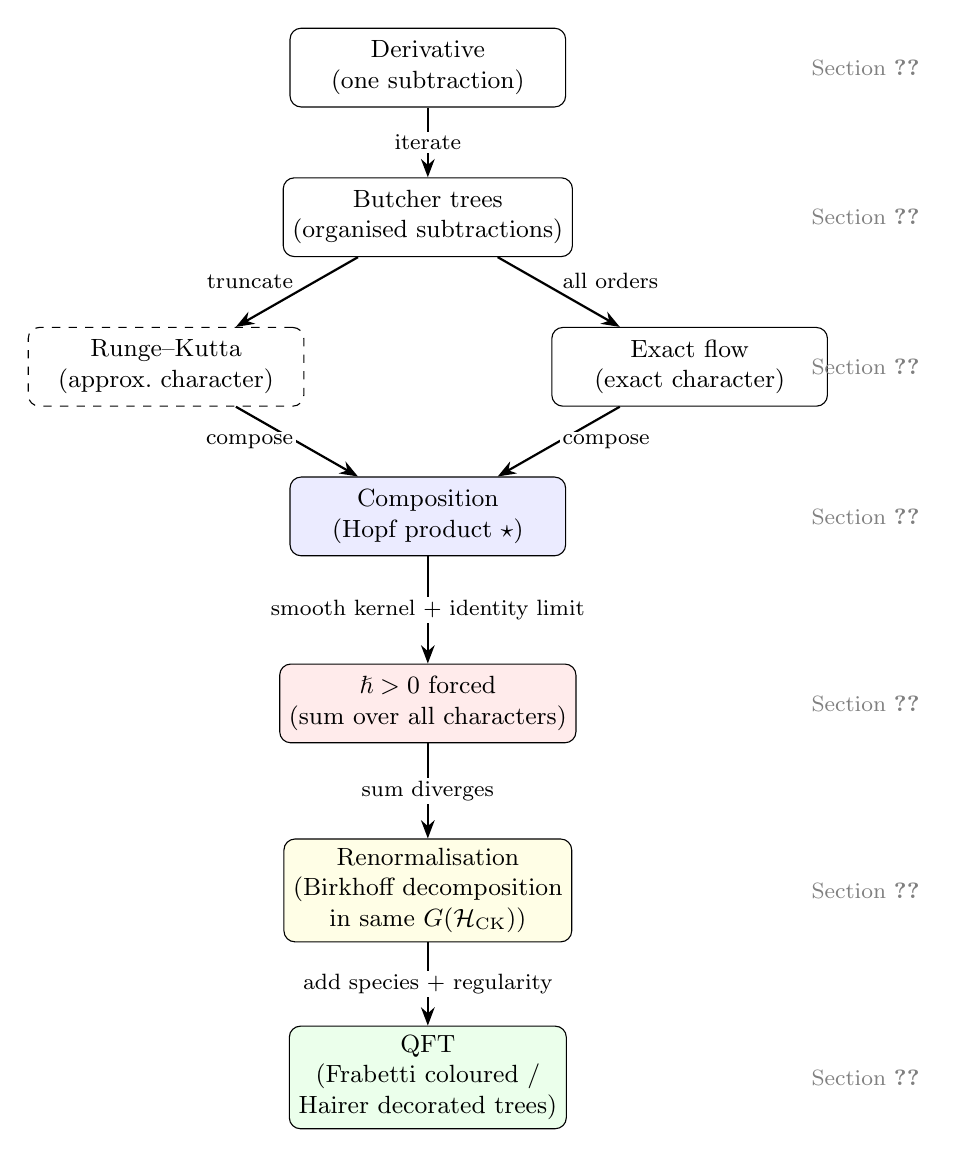
\begin{tikzpicture}[
  box/.style={draw, rounded corners, minimum width=3.5cm, minimum height=1cm,
    align=center, font=\small},
  arrow/.style={->, thick, >=Stealth},
  label/.style={font=\footnotesize, midway, fill=white, inner sep=1pt},
  scale=0.95
]

% Nodes
\node[box] (deriv) at (0,6) {Derivative\\(one subtraction)};
\node[box] (trees) at (0,4) {Butcher trees\\(organised subtractions)};
\node[box, dashed] (rk) at (-3.5,2) {Runge--Kutta\\(approx.\ character)};
\node[box] (exact) at (3.5,2) {Exact flow\\(exact character)};
\node[box, fill=blue!8] (comp) at (0,0) {Composition\\(Hopf product $\star$)};
\node[box, fill=red!8] (hbar) at (0,-2.5) {$\hbar > 0$ forced\\(sum over all characters)};
\node[box, fill=yellow!10] (renorm) at (0,-5) {Renormalisation\\(Birkhoff decomposition\\in same $\GH$)};
\node[box, fill=green!8] (qft) at (0,-7.5) {QFT\\(Frabetti coloured /\\Hairer decorated trees)};

% Arrows
\draw[arrow] (deriv) -- (trees) node[label] {iterate};
\draw[arrow] (trees) -- (rk) node[label, above left] {truncate};
\draw[arrow] (trees) -- (exact) node[label, above right] {all orders};
\draw[arrow] (rk) -- (comp) node[label, left] {compose};
\draw[arrow] (exact) -- (comp) node[label, right] {compose};
\draw[arrow] (comp) -- (hbar) node[label] {smooth kernel $+$ identity limit};
\draw[arrow] (hbar) -- (renorm) node[label] {sum diverges};
\draw[arrow] (renorm) -- (qft) node[label] {add species $+$ regularity};

% Side annotations
\node[font=\footnotesize, text=gray, anchor=west] at (5,6) {Section~\ref{sec:derivative}};
\node[font=\footnotesize, text=gray, anchor=west] at (5,4) {Section~\ref{sec:trees}};
\node[font=\footnotesize, text=gray, anchor=west] at (5,2) {Section~\ref{sec:exact-flow}};
\node[font=\footnotesize, text=gray, anchor=west] at (5,0) {Section~\ref{sec:coproduct}};
\node[font=\footnotesize, text=gray, anchor=west] at (5,-2.5) {Section~\ref{sec:quantization}};
\node[font=\footnotesize, text=gray, anchor=west] at (5,-5) {Section~\ref{sec:coproduct}};
\node[font=\footnotesize, text=gray, anchor=west] at (5,-7.5) {Section~\ref{sec:extensions}};

\end{tikzpicture}
\caption{%
  The cornerstone diagram.
  The entire chain --- from the derivative as a single subtraction
  to QFT renormalisation --- is organised by the same Hopf algebra
  $\HCK$.
  Each downward arrow adds compositional complexity;
  the algebraic structure (coproduct, characters, group law) remains
  the same throughout.
}
\label{fig:cornerstone-diagram}
\end{figure}


%% ===================================================================
\section{Honest gaps and open problems}
\label{sec:gaps}
%% ===================================================================

\subsection{The tree decoration problem}

In the ODE/B-series setting, trees are decorated by elementary
differentials $F(\tau)$ --- patterns of derivatives of the vector
field $f$.
In the QFT/Feynman setting, trees are decorated by residues of
Feynman diagrams --- patterns of propagators and vertices.

Brouder's theorem establishes that the \emph{undecorated} Hopf
algebras are isomorphic.
But the identification ``which ODE tree $\leftrightarrow$ which
Feynman diagram'' depends on the specific theory.

\begin{example}[Where the identification is explicit]
  For the 1D anharmonic oscillator
  $\ddot{x} + x + \lambda x^3 = 0$,
  written as a system $\dot{y} = f(y)$ with
  $f(x,v) = (v,\,-x-\lambda x^3)$:
  \begin{itemize}
    \item The B-series trees of $f$ map directly to the
      Feynman diagrams of $\phi^4$ in $0{+}1$ dimensions.
    \item The $|\tau|=2$ tree gives the one-loop correction.
    \item The $|\tau|=3$ trees give two-loop corrections.
  \end{itemize}
  In this case, the identification is canonical.
\end{example}

\begin{gap}[General theories]
  For gauge theories (QED, QCD), the tree structure is more complex:
  coloured/planar trees (Frabetti), with non-commutative Hopf algebra.
  The identification with B-series is indirect.
\end{gap}

\subsection{Path roughness}

\begin{gap}[Non-perturbative paths]
  The path integral sums over Wiener paths, which are
  H\"older-$1/2$ (not~$C^\infty$).
  A generic path does not have a B-series expansion.
  The tree-algebraic description applies to the
  \textbf{perturbative} expansion of the propagator
  (loop expansion in powers of $\hbar$ or couplings),
  not to individual paths.

  The honest statement is therefore:
  \begin{quote}
    The perturbative quantum propagator and the perturbative ODE
    solution (B-series) are organised by the same Hopf algebra.
    Quantisation, at the perturbative level, is the passage from
    one character to a sum over characters.
  \end{quote}
  Non-perturbative content (tunnelling, instantons, resurgence)
  lies beyond the tree algebra.
  The main paper's Remark H6.3 discusses partial recovery via
  Borel resummation.
\end{gap}

\subsection{The ``quantisation = extending the domain'' claim}

A possible precise formulation:

\begin{quote}
  Quantisation is a functor from $\GH$ (the Butcher group of
  single-character flows) to $\mathrm{Meas}(\GH)$ (measures on
  the Butcher group, i.e., weighted sums of characters).
  The parameter $\hbar$ controls the concentration of these measures:
  $\hbar\to 0$ gives a delta-measure on $\phi_{\mathrm{exact}}$;
  finite $\hbar$ gives a spread measure.
\end{quote}

This formulation has not been proved.
It would require:
\begin{enumerate}[label=(\alph*)]
  \item A rigorous definition of ``measure on $\GH$'' (the Butcher
    group is an infinite-dimensional pro-unipotent group).
  \item A proof that the path-integral measure, restricted to its
    perturbative sector, defines such a measure.
  \item A characterisation of $\hbar$ as the variance parameter.
\end{enumerate}


%% ===================================================================
\section{Extensions: coloured and decorated trees}
\label{sec:extensions}
%% ===================================================================

\subsection{Frabetti coloured trees (2000--2008)}

For QED, which has two propagator types (electron, photon),
Brouder and Frabetti constructed a \textbf{non-commutative}
Hopf algebra on \textbf{planar binary trees}, with one tree
species per propagator type.

\begin{figure}[ht]
\centering
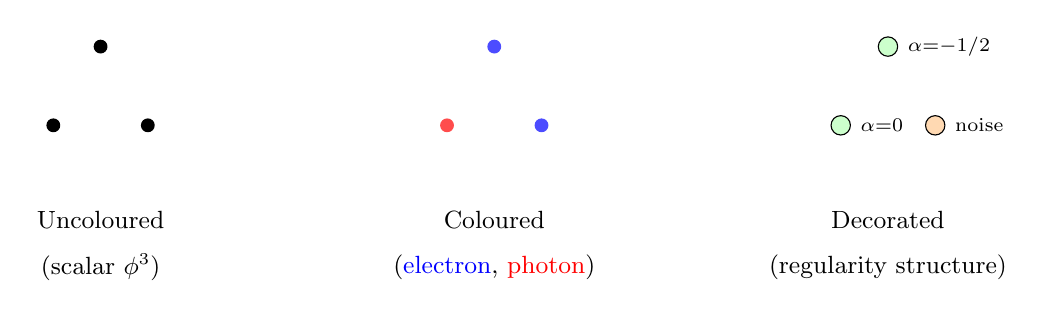
\begin{tikzpicture}[
  level distance=10mm,
  sibling distance=12mm,
  edge from parent/.style={thick}
]

% Uncoloured tree
\begin{scope}[xshift=0cm]
  \node[treenode] {}
    child { node[treenode] {} }
    child { node[treenode] {} };
  \node[font=\small] at (0,-2.2) {Uncoloured};
  \node[font=\small] at (0,-2.8) {(scalar $\phi^3$)};
\end{scope}

% Coloured tree: electron + photon
\begin{scope}[xshift=5cm]
  \node[circle, fill=blue!70, inner sep=0pt, minimum size=5pt] {}
    child[edge from parent/.style={thick, blue}] {
      node[circle, fill=red!70, inner sep=0pt, minimum size=5pt] {}
    }
    child[edge from parent/.style={thick, red, dashed}] {
      node[circle, fill=blue!70, inner sep=0pt, minimum size=5pt] {}
    };
  \node[font=\small] at (0,-2.2) {Coloured};
  \node[font=\small] at (0,-2.8) {(\textcolor{blue}{electron}, \textcolor{red}{photon})};
\end{scope}

% Decorated tree: Hairer
\begin{scope}[xshift=10cm]
  \node[circle, draw, fill=green!20, inner sep=1pt, minimum size=7pt,
    label=right:{\scriptsize $\alpha{=}{-}1/2$}] {}
    child[edge from parent/.style={thick, green!50!black}] {
      node[circle, draw, fill=green!20, inner sep=1pt, minimum size=7pt,
        label=right:{\scriptsize $\alpha{=}0$}] {}
    }
    child[edge from parent/.style={thick, green!50!black, decorate,
      decoration={zigzag,segment length=3pt,amplitude=1pt}}] {
      node[circle, draw, fill=orange!30, inner sep=1pt, minimum size=7pt,
        label=right:{\scriptsize noise}] {}
    };
  \node[font=\small] at (0,-2.2) {Decorated};
  \node[font=\small] at (0,-2.8) {(regularity structure)};
\end{scope}

\end{tikzpicture}
\caption{%
  Three levels of tree structure.
  \textbf{Left:} Butcher/Connes--Kreimer uncoloured trees
  (commutative Hopf algebra, scalar ODE/QFT).
  \textbf{Centre:} Frabetti coloured planar trees
  (non-commutative, gauge theories with multiple propagator types).
  \textbf{Right:} Hairer decorated trees
  (regularity structures, singular SPDEs;
  vertices carry regularity exponents, edges may carry noise type).
}
\label{fig:three-levels}
\end{figure}

In the ODE analogy, coloured trees correspond to systems with
multiple coupling types:
$\dot{y}_i = f_i(y_1,\ldots,y_n)$ where the $f_i$ depend on
the $y_j$ in structurally different ways.

\textbf{Status:} the algebraic structure is proved.
The physical payoff was limited: Frabetti confirmed that
Connes--Kreimer extends to gauge theories but did not simplify
calculations.

\subsection{Hairer decorated trees (2014)}

For singular SPDEs (KPZ equation, $\Phi^4_3$), Hairer's
regularity structures use trees decorated with:
\begin{itemize}
  \item \textbf{Regularity exponents} at vertices
    (how singular the distribution is).
  \item \textbf{Noise types} on certain edges
    (stochastic forcing terms).
\end{itemize}

Bruned--Hairer--Zambotti (2019) proved that Hairer's BPHZ-type
renormalisation of regularity structures \emph{is} a Hopf-algebraic
renormalisation on decorated trees, with the same structural
coproduct as Connes--Kreimer.

In the cornerstone language:
\begin{itemize}
  \item \textbf{Butcher:} each vertex $=$ one smooth derivative
    (counterterm subtraction of a smooth function).
  \item \textbf{Hairer:} each vertex $=$ one distributional
    operation (counterterm subtraction of a distribution,
    which may not exist without renormalisation).
\end{itemize}

\subsection{The three-level hierarchy}

\begin{figure}[ht]
\centering
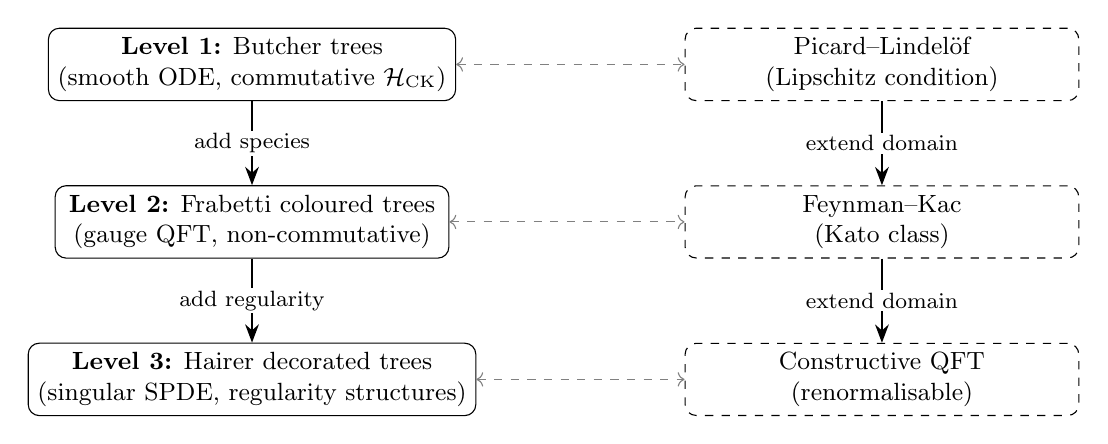
\begin{tikzpicture}[
  box/.style={draw, rounded corners, minimum width=5cm,
    minimum height=0.9cm, align=center, font=\small},
  arrow/.style={->, thick, >=Stealth},
  label/.style={font=\footnotesize, midway, fill=white, inner sep=1pt}
]

\node[box] (L1) at (0,3) {%
  \textbf{Level 1:} Butcher trees\\
  (smooth ODE, commutative $\HCK$)};

\node[box] (L2) at (0,1) {%
  \textbf{Level 2:} Frabetti coloured trees\\
  (gauge QFT, non-commutative)};

\node[box] (L3) at (0,-1) {%
  \textbf{Level 3:} Hairer decorated trees\\
  (singular SPDE, regularity structures)};

% Parallel column
\node[box, dashed] (P1) at (8,3) {%
  Picard--Lindel\"of\\
  (Lipschitz condition)};

\node[box, dashed] (P2) at (8,1) {%
  Feynman--Kac\\
  (Kato class)};

\node[box, dashed] (P3) at (8,-1) {%
  Constructive QFT\\
  (renormalisable)};

\draw[arrow] (L1) -- (L2) node[label] {add species};
\draw[arrow] (L2) -- (L3) node[label] {add regularity};

\draw[arrow] (P1) -- (P2) node[label] {extend domain};
\draw[arrow] (P2) -- (P3) node[label] {extend domain};

\draw[<->, dashed, gray] (L1) -- (P1);
\draw[<->, dashed, gray] (L2) -- (P2);
\draw[<->, dashed, gray] (L3) -- (P3);

\end{tikzpicture}
\caption{%
  The three-level tree hierarchy (left) mirrors the paper's
  well-posedness hierarchy (right).
  At each level, the tree algebra becomes richer
  (coloured, then decorated) and the domain of well-posedness
  extends (Lipschitz $\subset$ Kato $\subset$ renormalisable).
}
\label{fig:hierarchy}
\end{figure}


%% ===================================================================
\section{Implications for the main paper}
\label{sec:implications}
%% ===================================================================

\subsection{The missing section}

The main paper's Section~8 presents D6.2a (control map) and H6.2
(rooted-tree bookkeeping) as an \emph{analogy} between Runge--Kutta
and renormalisation.
The cornerstone says it is an \emph{identity}.

A new subsection (8.7 or equivalent) should state:
\begin{enumerate}
  \item The exact flow is the fully renormalised character of $\HCK$.
  \item Numerical methods are approximate characters; order conditions
    $=$ tree-by-tree matching.
  \item The control map $\tau_b$ is the counterterm at $|\tau|=2$.
  \item Quantisation extends from one character to all characters.
  \item $\hbar > 0$ is forced by composition $+$ identity (P4.2).
  \item Renormalisation handles divergences using the same coproduct.
\end{enumerate}

\subsection{What it would prove}

If made fully precise (resolving the gaps of Section~\ref{sec:gaps}),
this would establish:

\begin{quote}
  \textbf{Quantisation is the compositional completion of the
  counterterm-subtraction algebra.}
\end{quote}

Classical mechanics uses one character.
Quantum mechanics uses all characters.
The passage is forced by requiring smooth composition with identity.
Renormalisation controls the extension.
Derivative, quantisation, and renormalisation are three instances
of the same algebraic operation (counterterm subtraction organised
by rooted trees) at increasing levels of compositional complexity.

This is the main paper's thesis --- refinement-compatibility forces
the chain Newton $\to$ quantum $\to$ QFT --- stated in its most
algebraic form.


%% ===================================================================
\section*{References}
%% ===================================================================

\begin{enumerate}[label={[\arabic*]}]
  \item J.~C.~Butcher,
    ``An algebraic theory of integration methods,''
    \emph{Math.\ Comp.}\ \textbf{26} (1972), 79--106.

  \item Ch.~Brouder,
    ``Runge--Kutta methods and renormalization,''
    \emph{Eur.\ Phys.\ J.\ C}\ \textbf{12} (2000), 521--534;
    arXiv:\texttt{hep-th/9904014}.

  \item A.~Connes and D.~Kreimer,
    ``Renormalization in QFT and the Riemann--Hilbert problem~I,''
    \emph{Comm.\ Math.\ Phys.}\ \textbf{210} (2000), 249--273.

  \item Ch.~Brouder and A.~Frabetti,
    ``Noncommutative renormalization for massless QED,''
    arXiv:\texttt{hep-th/0011161} (2000).

  \item Ch.~Brouder and A.~Frabetti,
    ``QED Hopf algebras on planar binary trees,''
    \emph{J.\ Algebra}\ \textbf{267} (2003), 298--322;
    arXiv:\texttt{math/0112043}.

  \item A.~Frabetti,
    ``Groups of tree-expanded series,''
    \emph{J.\ Algebra}\ \textbf{319} (2008), 377--413.

  \item A.~Frabetti and D.~Manchon,
    ``Five interpretations of Fa\`a di Bruno's formula,''
    arXiv:\texttt{1402.5551} (2014).

  \item M.~Hairer,
    ``A theory of regularity structures,''
    \emph{Inventiones Math.}\ \textbf{198} (2014), 269--504.

  \item Y.~Bruned, M.~Hairer, and L.~Zambotti,
    ``Algebraic renormalisation of regularity structures,''
    \emph{Inventiones Math.}\ \textbf{215} (2019), 1039--1156.

  \item E.~Hairer, C.~Lubich, and G.~Wanner,
    \emph{Geometric Numerical Integration}
    (2nd ed., Springer, 2006).

  \item G.~Soderlind,
    ``The logarithmic norm: history and modern theory,''
    \emph{BIT Numerical Mathematics}\ \textbf{46} (2006), 631--652.

  \item Ch.~Brouder,
    ``Trees, renormalization and differential equations,''
    \emph{BIT Numerical Mathematics}\ \textbf{44} (2004), 425--438.
\end{enumerate}

\end{document}
